\documentclass[a4paper,12pt]{article}

\usepackage[left=1.5cm,text={18cm, 25cm},top=2.5cm]{geometry}
\usepackage[IL2]{fontenc}
\usepackage[czech]{babel}
\usepackage[T1]{fontenc}
\usepackage{graphics}
\usepackage{hyperref}
\usepackage{amsthm}
\usepackage{float}

\setlength\parindent{0pt}

\begin{document}

\begin{figure}[h]
\centering
\scalebox{0.15}{
\includegraphics{logo_cz.png}}
\end{figure}

\vspace{\stretch{0.882}}
\begin{center}
\Huge \textbf{Dokumentace k projektu}\\
\Large ISS/VSG Projekt 2021/22

\vspace{\stretch{0.758}}
\vspace{\stretch{0.15}}

\end{center}
\mbox{}
\vfill
{\large\today}
\hfill
Novák David (xnovak2r)
\thispagestyle{empty}
\newpage

\tableofcontents
\thispagestyle{empty}
\newpage

\section{Úvod}
Cílem projektu bylo analyzovat zadaný signál a nalézt čtyři harmonicky vztažené cosinusovky, které do něj byli přidány. Poté vytvořit filtr/y a ten/ty následně použít pro filtraci daného signálu. Tento projekt je řešen v jazyce Python. K výpočtům dopomohly funkce z knihoven \emph{numpy} a \emph{scipy}, pro tvorbu grafů byla využita knihovna \emph{matplotlib}.

\section{Otázky}
\subsection{Otázka 1}
Délka signálu:
\begin{itemize}
	\item ve vzorcích: 54170
	\item v sekundách: 3.385625 sekund
\end{itemize}
Minimální hodnota: -0.100738525390625\\
Maximální hodnota: 0.127197265625\\
\begin{figure}[h]
\centering
\scalebox{0.95}{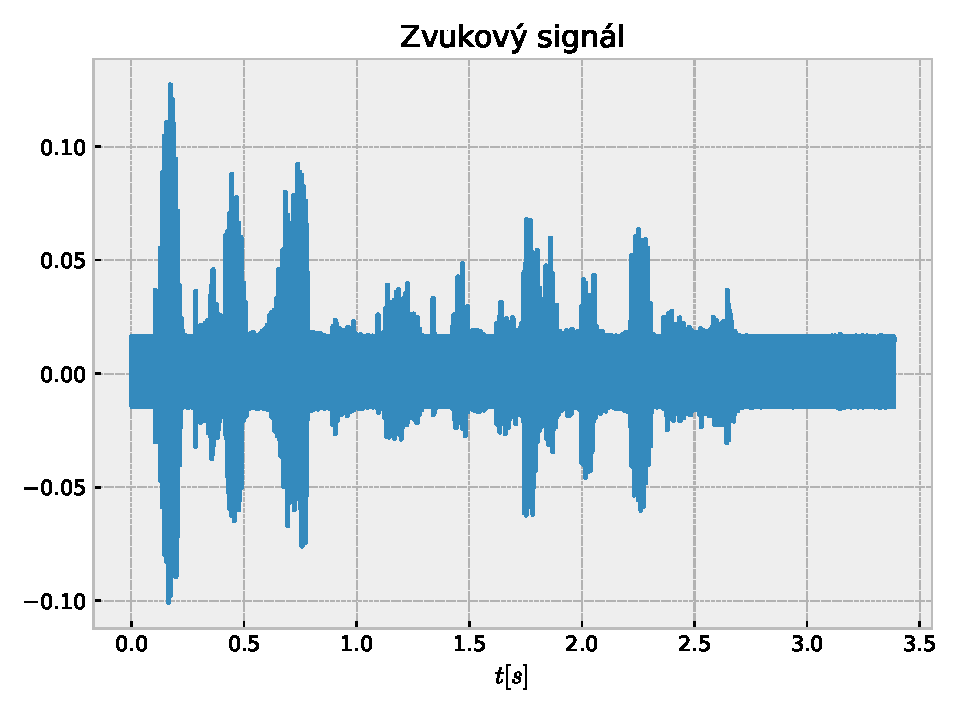
\includegraphics{plots/plot_1.pdf}}
\end{figure}
\\
Pro získání údajů byl využit modul \emph{wavfile} s postumem dle Jupyter notebooku.

\subsection{Otázka 2}
\begin{figure}[h]
\centering
\scalebox{1}{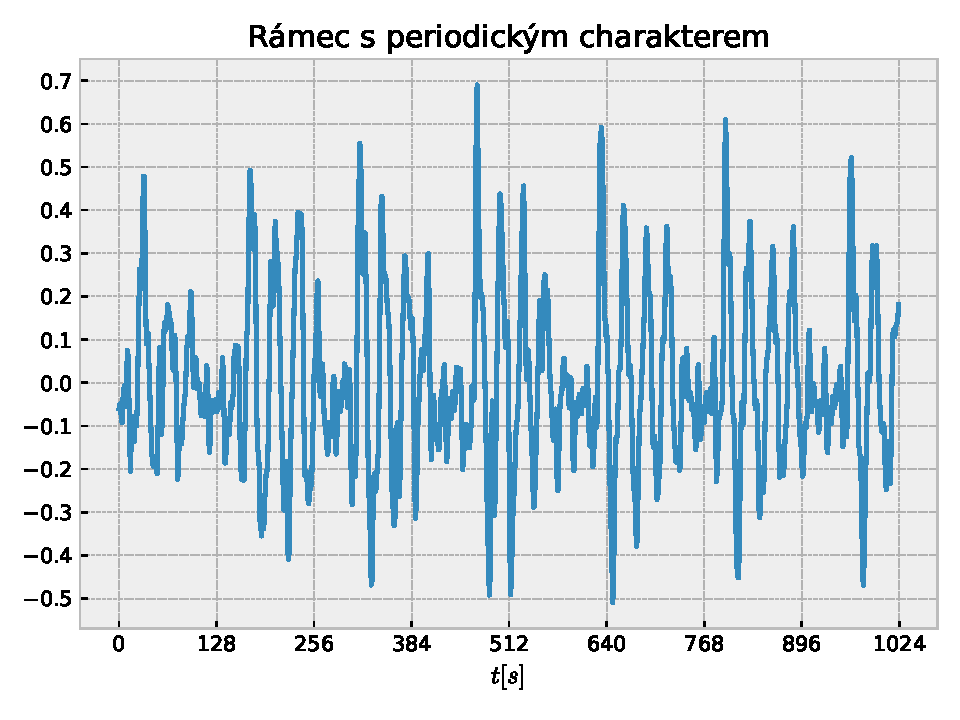
\includegraphics{plots/plot_2.pdf}}
\end{figure}
Dle zadání byl signál ustředněn a normalizován. Do řádků matice byly postupně uloženy jednotlivé úseky pomocí jednoduchého while cyklu. Celá matice byla nakonec transponována. Pro zobrazení byl vybrán 14. rámec.

\subsection{Otázka 3}
\begin{figure}[h]
\centering
\scalebox{1}{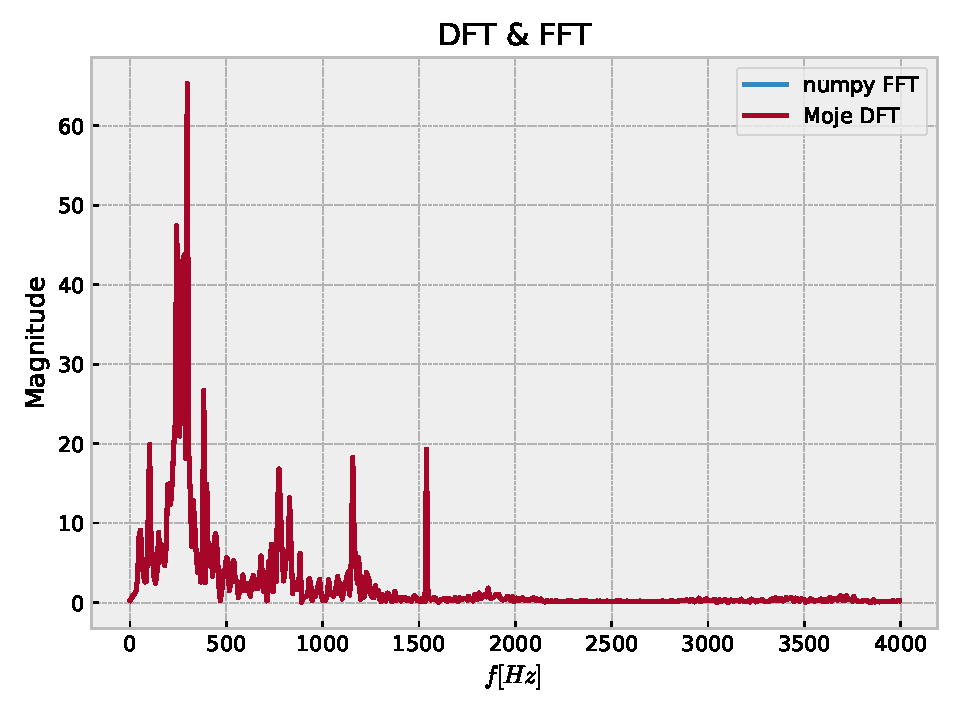
\includegraphics{plots/plot_3.pdf}}
\end{figure}
DFT funguje správně, o čemž se lze přesvědčit srovnáním s \emph{numpy} FFT. Bohužel z důvodu implementace (implementováno vnořenými while cykly), trvá DFT dlouho. Při snaze o před počítání části výrazu před while cykly docházelo k transformaci z komplexního čísla s čistě imaginární složkou na komplexní číslo s reálnou a imaginární složkou. Po neschopnosti opravy tohoto problému byl proto zvolen tento jednodušší, byť značně pomalejší způsob.

\newpage
\subsection{Otázka 4}
\begin{figure}[h!]
\scalebox{0.9}{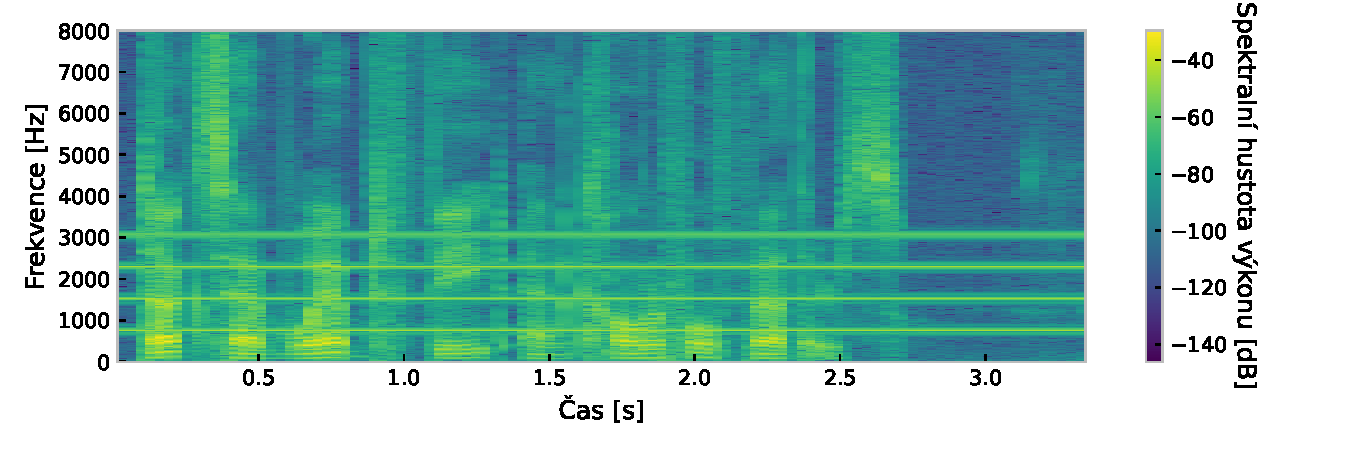
\includegraphics{plots/plot_4.pdf}}
\end{figure}
Pro postup při tvorbě spektrogramu byl využit postupem z Jupyter notebooku.

\newpage
\subsection{Otázka 5}
Rušivé frekvence:
\begin{itemize}
	\item frekvence 1: 650 Hz
	\item frekvence 2: 1300 Hz
	\item frekvence 3: 1950 Hz
	\item frekvence 4: 2600 Hz
\end{itemize}
Frekvence byly nalezeny ručně vytvořením spektrogramu s menšími kroky na frekvenční ose a přidáním dobře viditelné mřížky na oné ose. 

\subsection{Otázka 6}
\begin{figure}[h]
\centering
\scalebox{1}{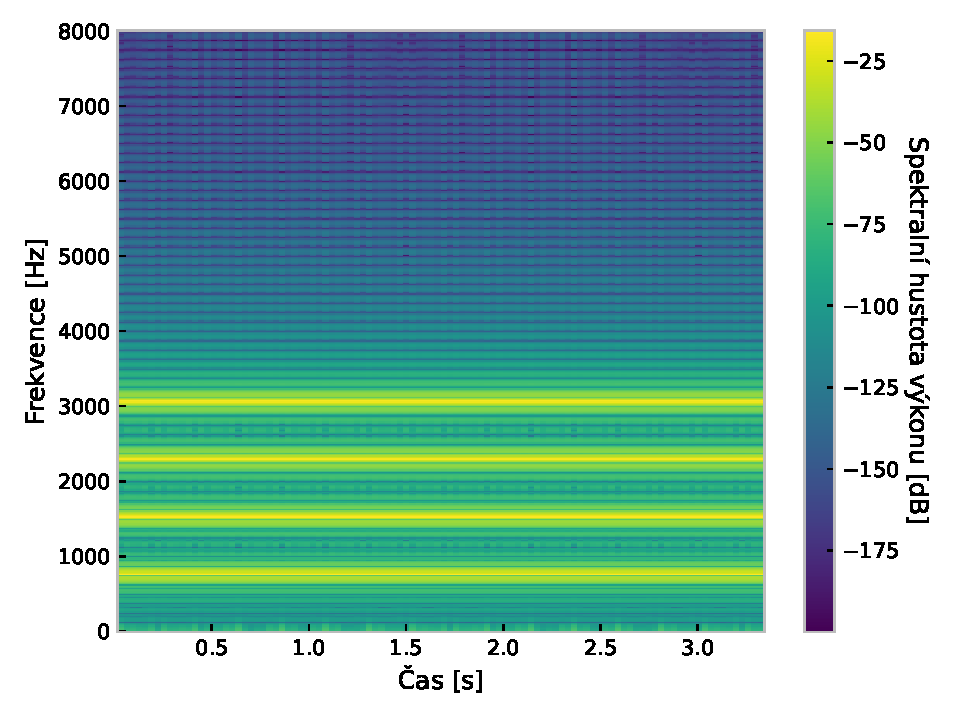
\includegraphics{plots/plot_6.pdf}}
\end{figure}
Po vygenerování cosinusovek s frekvencemi uvedenými v otázce 5, jejich poslechu a následné panice, bylo zjištěno, že při vygenerování cosinusovek o čtyřnásobné frekvenci vzniknou požadované cosinusovky. Tento signál zní a vypadá stejně, pouze je hlasitější. Pro vygenerování cosinusovek byla využita funkce \emph{cos} z knihovny \emph{numpy}. Pro jejich zápis byl opět využit modul \emph{wavfile}.

\newpage
\subsection{Otázka 7.3}
Impulzní odezvy filtrů:
\begin{figure}[h!]
\centering
\begin{minipage}{0.48\textwidth}
\scalebox{0.6}{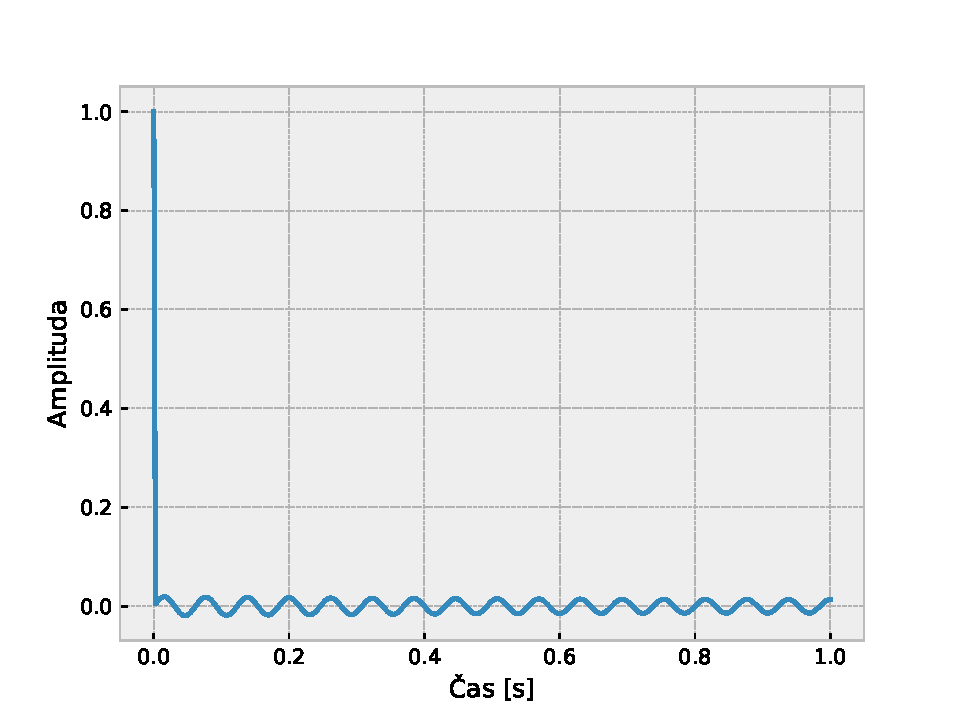
\includegraphics{plots/plot_7.1.pdf}}
\caption{Filtr 1}
\end{minipage}
\hfill 
\begin{minipage}{0.48\textwidth}
\scalebox{0.6}{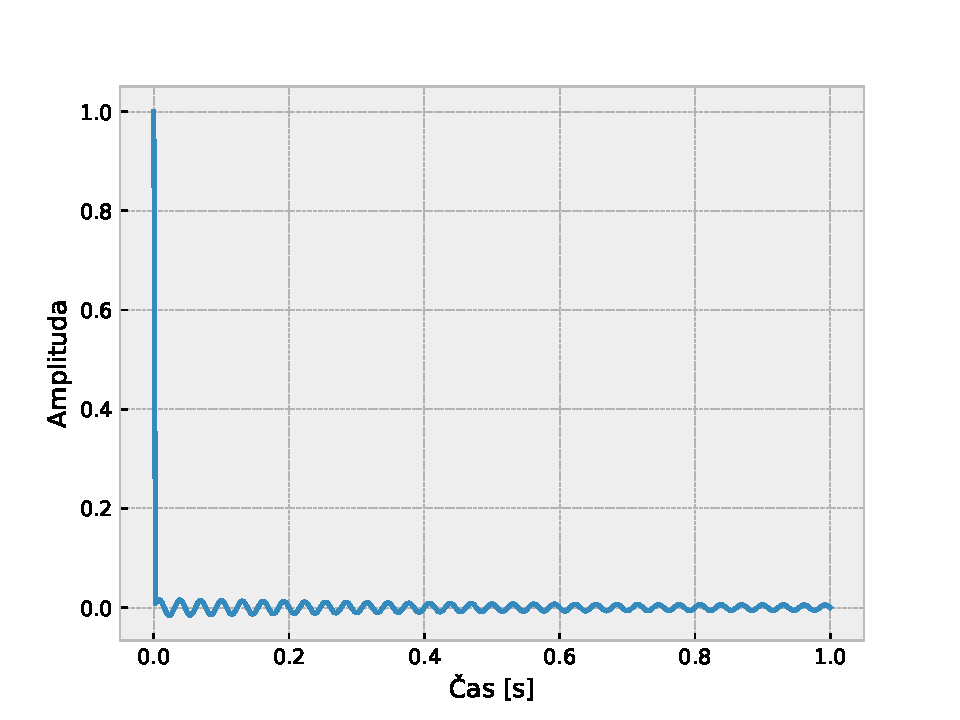
\includegraphics{plots/plot_7.2.pdf}}
\caption{Filtr 2}
\end{minipage}
\end{figure}

\begin{figure}[h!]
\centering
\begin{minipage}{0.48\textwidth}
\scalebox{0.6}{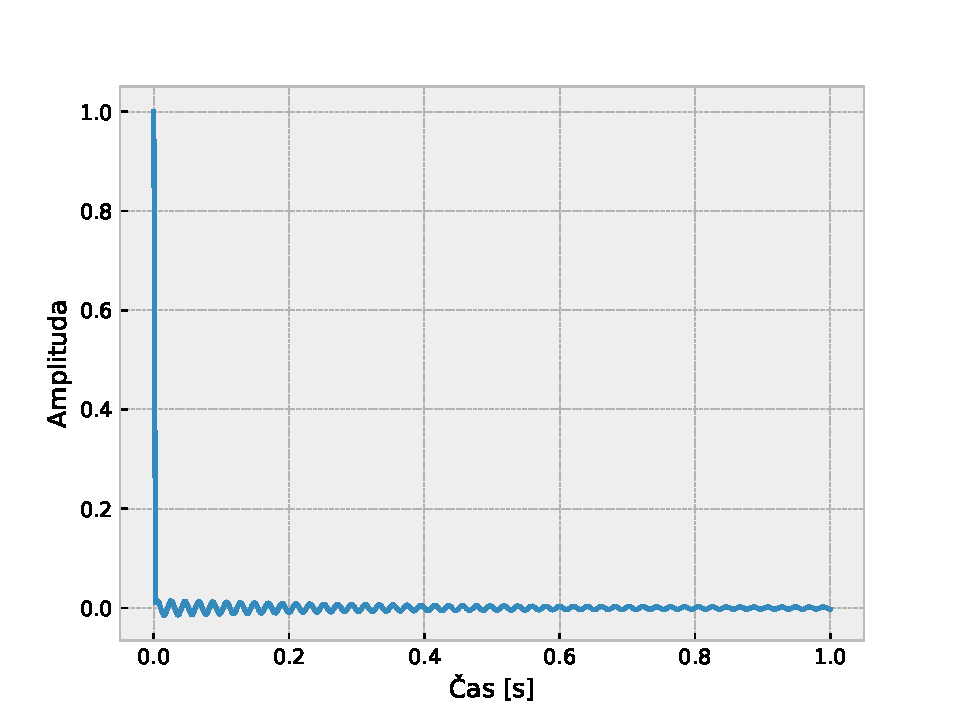
\includegraphics{plots/plot_7.3.pdf}}
\caption{Filtr 3}
\end{minipage}
\hfill 
\begin{minipage}{0.48\textwidth}
\scalebox{0.6}{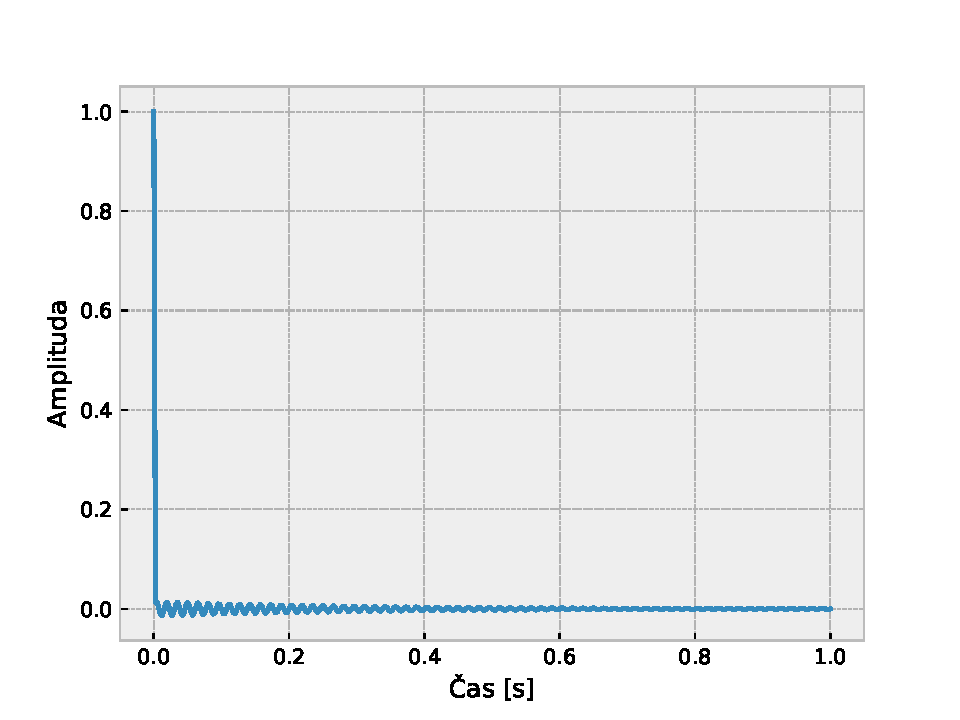
\includegraphics{plots/plot_7.4.pdf}}
\caption{Filtr 4}
\end{minipage}
\end{figure}

Po neúspěšných pokusech o vytvoření filtrů pomocí funkce \emph{butter} z knihovny \emph{signal} byla pro tvorbu filtrů využita funkce \emph{iirnotch} z téže knihovny.

\newpage
\subsection{Otázka 8}
\begin{figure}[h!]
\centering
\scalebox{0.8}{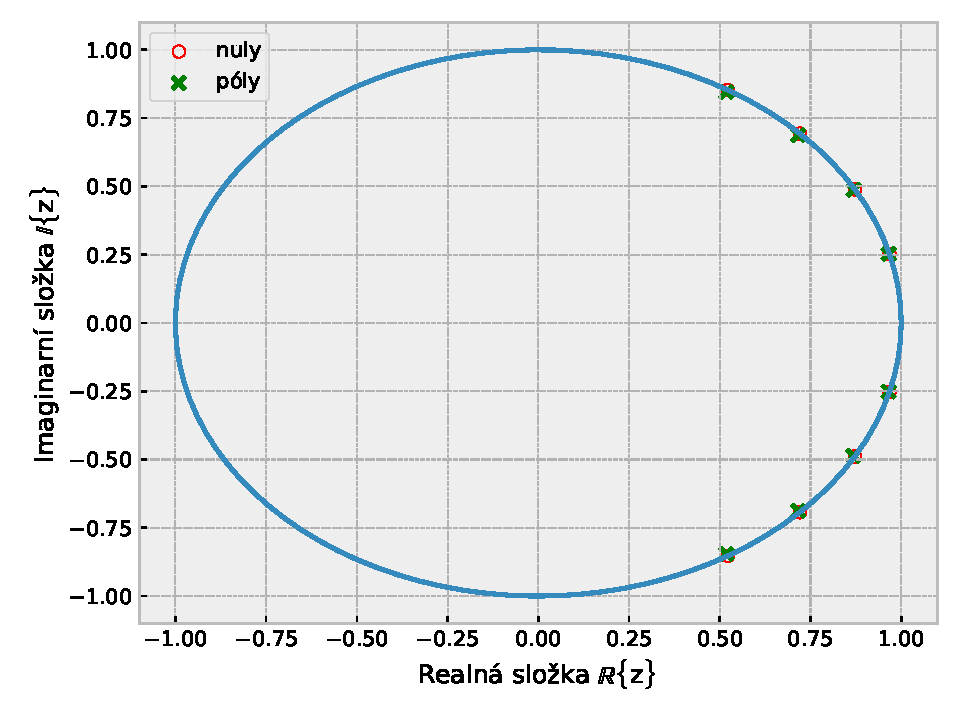
\includegraphics{plots/plot_8.pdf}}
\end{figure}

U této otázky byl opět využit postup z Jupyter notebooku.

\subsection{Otázka 9}
Frekvenční charakteristiky byly vytvořeny s pomocí oficiální \emph{scipy} stránky pro funkci \emph{iirnotch}.
\begin{figure}[h!]
\centering
\begin{minipage}{0.48\textwidth}
\scalebox{0.6}{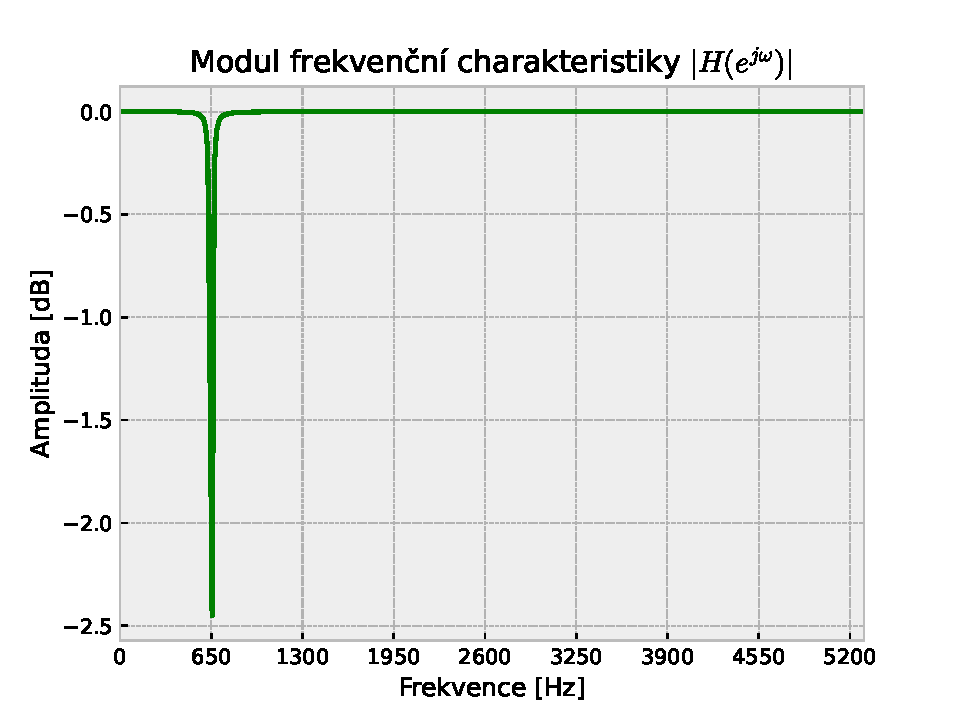
\includegraphics{plots/plot_9.1.pdf}}
\end{minipage}
\hfill 
\begin{minipage}{0.48\textwidth}
\scalebox{0.6}{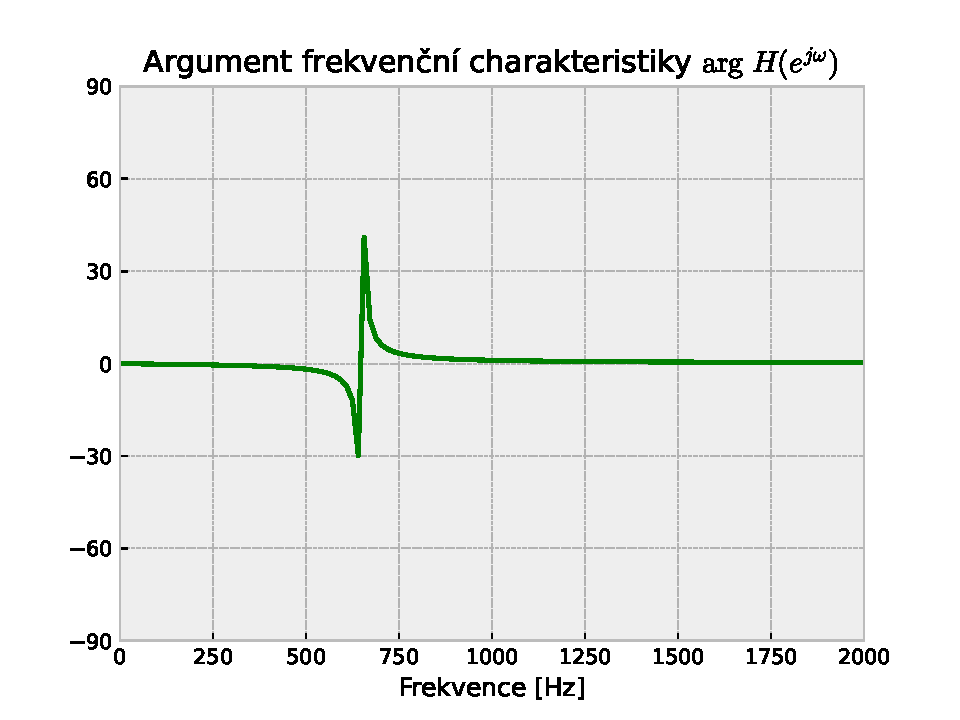
\includegraphics{plots/plot_9.2.pdf}}
\end{minipage}
\caption{Filtr 1}
\end{figure}

\begin{figure}[h!]
\centering
\begin{minipage}{0.48\textwidth}
\scalebox{0.6}{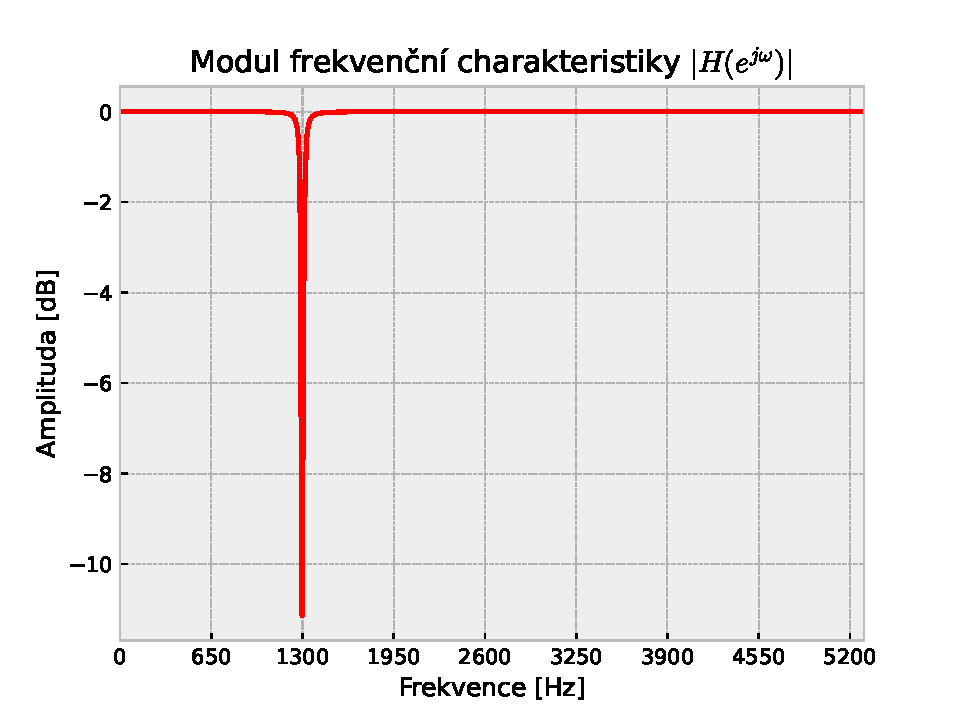
\includegraphics{plots/plot_9.3.pdf}}
\end{minipage}
\hfill 
\begin{minipage}{0.48\textwidth}
\scalebox{0.6}{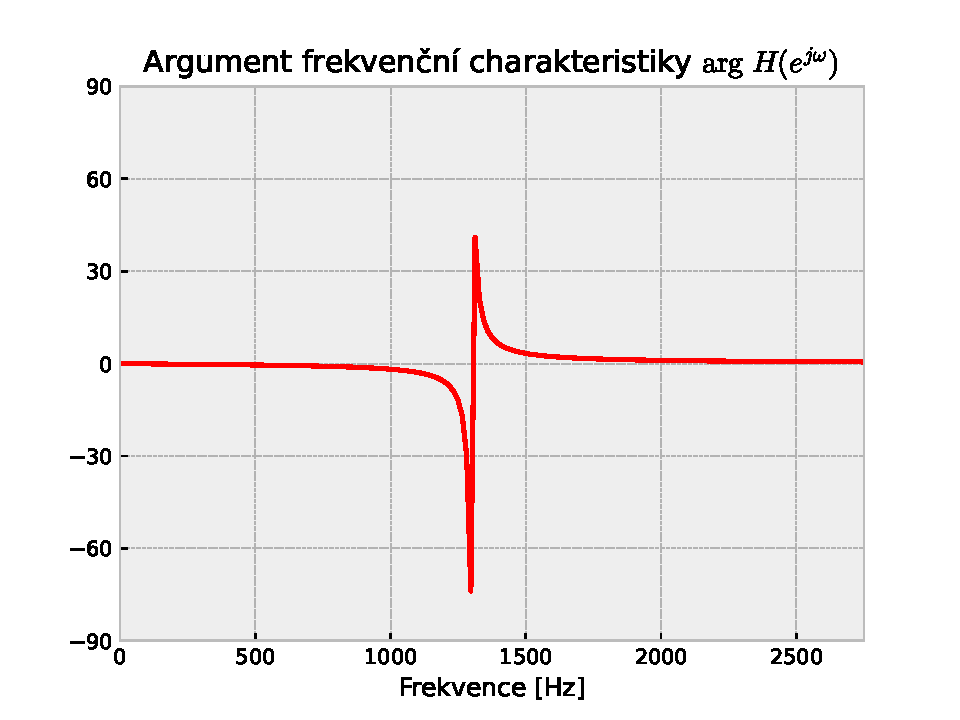
\includegraphics{plots/plot_9.4.pdf}}
\end{minipage}
\caption{Filtr 2}
\end{figure}

\begin{figure}[h!]
\centering
\begin{minipage}{0.48\textwidth}
\scalebox{0.6}{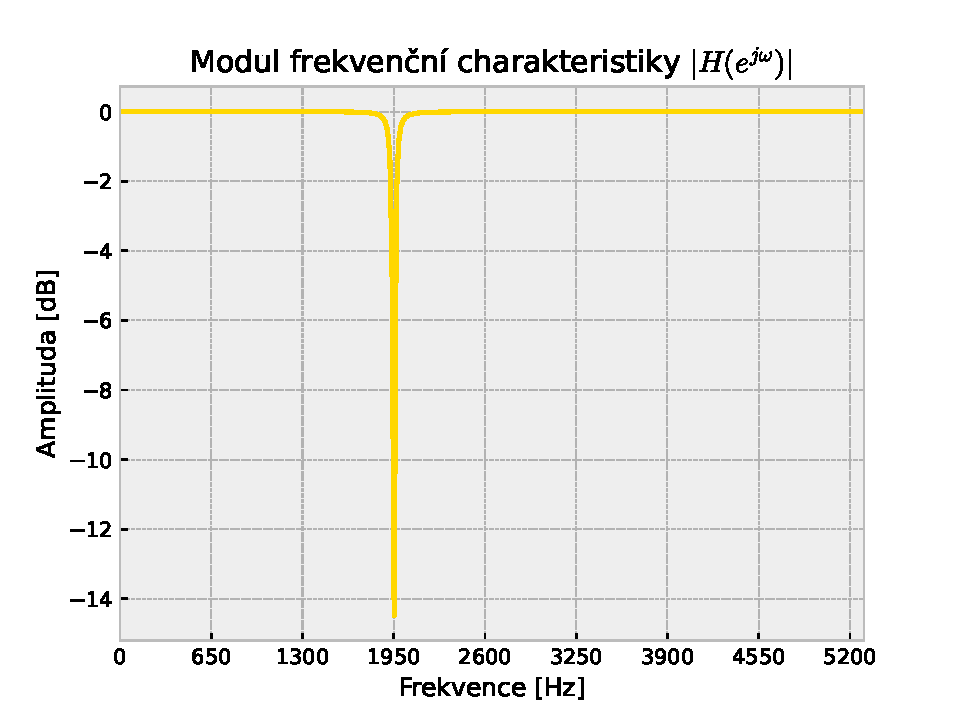
\includegraphics{plots/plot_9.5.pdf}}
\end{minipage}
\hfill 
\begin{minipage}{0.48\textwidth}
\scalebox{0.6}{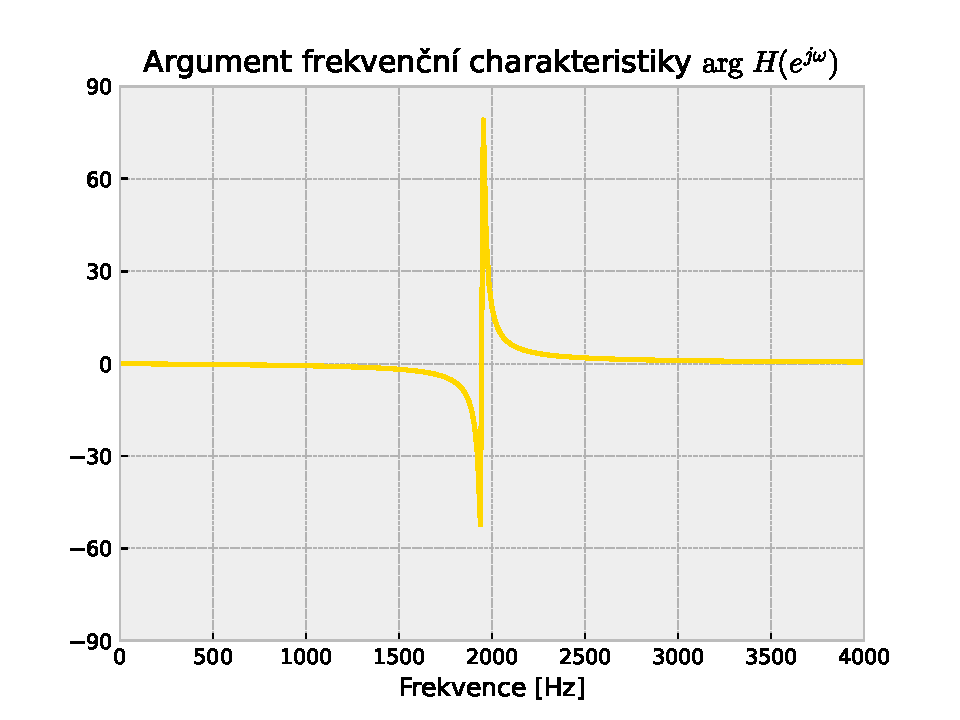
\includegraphics{plots/plot_9.6.pdf}}
\end{minipage}
\caption{Filtr 3}
\end{figure}

\begin{figure}[H]
\centering
\begin{minipage}{0.48\textwidth}
\scalebox{0.6}{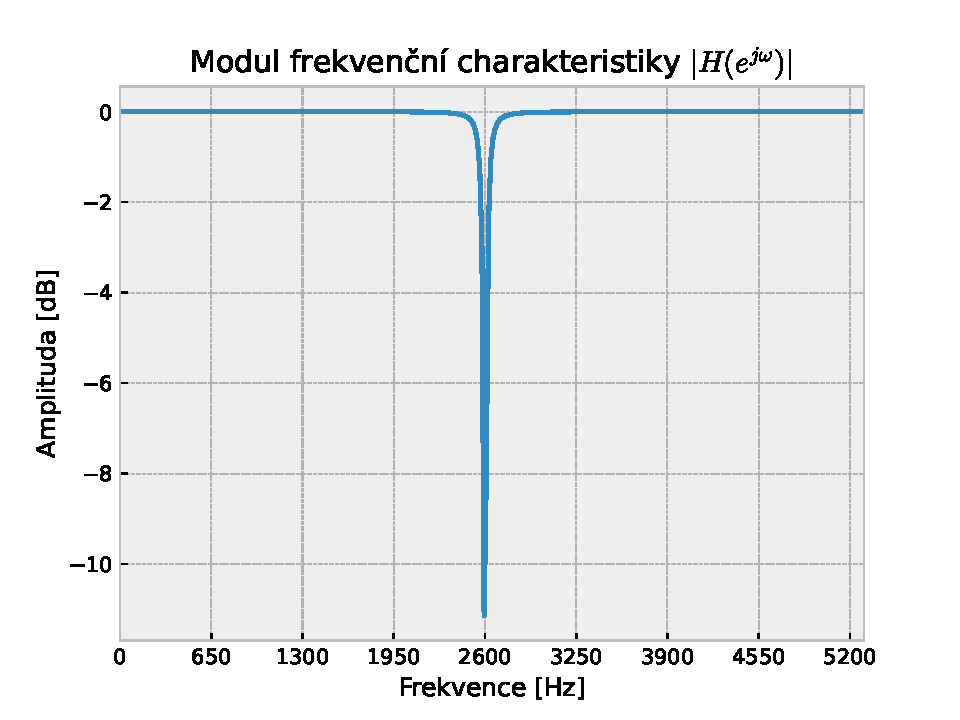
\includegraphics{plots/plot_9.7.pdf}}
\end{minipage}
\hfill 
\begin{minipage}{0.48\textwidth}
\scalebox{0.6}{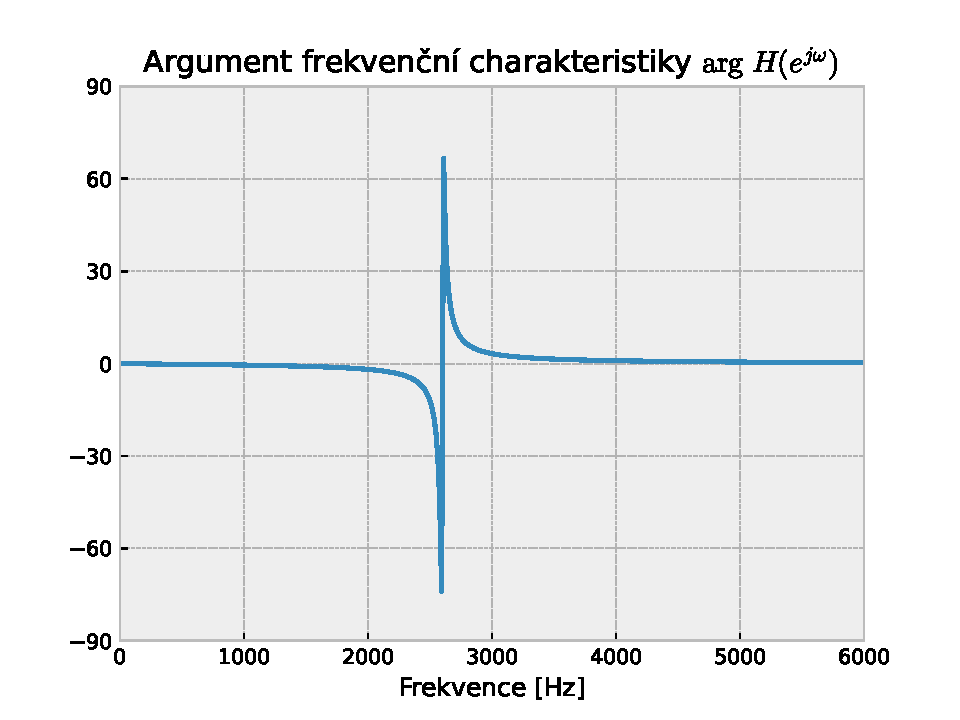
\includegraphics{plots/plot_9.8.pdf}}
\end{minipage}
\caption{Filtr 4}
\end{figure}

\newpage
\subsection{Otázka 10}
Filtrace signálu byla provedena pomocí funkce \emph{filtfilt} a filtru připraveného v předchozí části. Uloženy jsou znovu pomocí modulu \emph{wavfile}. Filtr však nesplňuje očekávané chování.

\section{Nestandardní zdroje}
V projektu byly mimo standardních stránek využity také stránky pro knihovnu \emph{numpy}, dále byly pro projekt využity oficiální \emph{scipy} stránky, zejména pak stránky pro funkce \emph{iirnotch}, \emph{freqz}, \emph{filtfilt}.

\end{document}
